
\chapter{Variables, expresiones y sentencias}

\section{Valores y tipos}

\index{valor} \index{tipo} \index{cadena}

Un \textbf{valor} es una de las cosas fundamentales—como una letra
o un número—que un programa manipula. Los valores que hemos visto
hasta ahorra son \texttt{2} (el resultado cuando añadimos \texttt{1
+ 1}, y {\verb+"Hola todo el Mundo!"+}.

Los valores pertenecen a diferentes \textbf{tipos}: \texttt{2} es
un entero, y {\verb+"Hola, Mundo!"+} es una \textbf{cadena}, llamada
así porque contiene una ``cadena'' de letras. Usted (y el intérprete)
pueden identificar cadenas porque están encerradas entre comillas.

La función de impresión también trabaja con enteros.

\inputencoding{latin9}\begin{lstlisting}
>>> print(4)
4
\end{lstlisting}
\inputencoding{utf8} 

Si no está seguro del tipo que un valor tiene, el intérprete le puede
decir.

\inputencoding{latin9}\begin{lstlisting}
>>> type("Hola, Mundo!")
str
>>> type(17)
int
\end{lstlisting}
\inputencoding{utf8} 

Sin despertar ninguna sorpresa, las cadenas pertenecen al tipo \texttt{\textbf{str}}\texttt{ing
(cadena)} y los enteros pertenecen al tipo \texttt{\textbf{int}}\texttt{eger}.
Menos obvio, los números con cifras decimales pertenecen a un tipo
llamado \texttt{float}, porque éstos se representan en un formato
denominado \textbf{punto flotante}.

\index{tipo} \index{cadena} \index{tipo!cadena} \index{int} \index{tipo!int}
\index{float} \index{tipo!float}

\inputencoding{latin9}\begin{lstlisting}
>>> type(3.2)
float
\end{lstlisting}
\inputencoding{utf8}
¿Qué ocurre con valores como {\verb+"17"+} y {\verb+"3.2"+}?
Parecen números, pero están encerrados entre comillas como las cadenas.

\inputencoding{latin9}\begin{lstlisting}
>>> type("17")
str
>>> type("3.2")
str
\end{lstlisting}
\inputencoding{utf8}
Ellos son cadenas.

Cuando usted digita un número grande, podría estar tentado a usar
comas para separar grupos de tres dígitos, como en \texttt{1,000,000}.
Esto no es un número entero legal en Python, pero esto si es legal:

\inputencoding{latin9}\begin{lstlisting}
>>> print(1,000,000)
1 0 0
\end{lstlisting}
\inputencoding{utf8}
¡Bueno, eso no es lo que esperábamos!. Resulta que \texttt{1,000,000}
es una tupla, algo que encontraremos en el Capítulo \ref{tuplechap}.
De momento, recuerde no poner comas en sus números enteros.

\section{Variables}

\index{variable} \index{asignación} \index{sentencia!asignación}

Una de las características más poderosas en un lenguaje de programación
es la capacidad de manipular \textbf{variables}. Una variable es un
nombre que se refiere a un valor.

La \textbf{sentencia de asignación} crea nuevas variables y les da
valores:

\inputencoding{latin9}\begin{lstlisting}
>>> mensaje = "�Qu� Onda?"
>>> n = 17
>>> pi = 3.14159
\end{lstlisting}
\inputencoding{utf8}
Este ejemplo hace tres asignaciones: la primera asigna la cadena {\verb+"¿Qué Onda?"+}
a una nueva variable denominada \texttt{mensaje}, la segunda le asigna
el entero \texttt{17} a \texttt{n} y la tercera le asigna el número
de punto flotante \texttt{3.14159} a \texttt{pi}.

\index{diagrama de estados}

Una manera común de representar variables en el papel es escribir
el nombre de la variable con una flecha apuntando a su valor. Esta
clase de dibujo se denomina \textbf{diagrama de estados} porque muestra
el estado de cada una de las variables (piense en los valores como
el estado mental de las variables). Este diagrama muestra el resultado
de las sentencias de asignación anteriores:

\beforefig \centerline{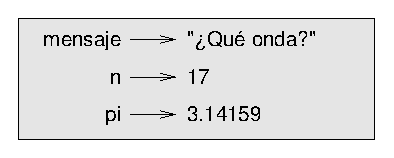
\includegraphics{illustrations/state2}}
\afterfig

La función \texttt{print} también funciona con variables.

\inputencoding{latin9}\begin{lstlisting}
>>> print(mensaje)
Que Onda?
>>> print(n)
17
>>> print(pi)
3.14159
\end{lstlisting}
\inputencoding{utf8} 

En cada caso el resultado es el valor de la variable. Las variables
también tienen tipos; nuevamente, le podemos preguntar al intérprete
cuales son.

\inputencoding{latin9}\begin{lstlisting}
>>> type(mensaje)
str
>>> type(n)
int
>>> type(pi)
float
\end{lstlisting}
\inputencoding{utf8} 

El tipo de una variable es el mismo del valor al que se refiere.

\section{Nombres de variables y palabras reservadas}

\index{palabra reservada} \index{palabra!reservada}

Los programadores, generalmente, escogen nombres significativos para
sus variables —que especifiquen para qué se usa la variable.

Estos nombres pueden ser arbitrariamente largos. Pueden contener letras
y números, pero tienen que empezar con una letra. Aunque es legal
usar letras mayúsculas, por convención no lo hacemos. Si usted lo
hace, recuerde que la capitalización importa, \texttt{Pedro} y \texttt{pedro}
son variables diferentes.

El carácter subrayado (\texttt{\_}) puede aparecer en un nombre. A
menudo se usa en nombres con múltiples palabras, tales como \texttt{mi\_nombre}
ó \texttt{precio\_del\_café\_en\_china}.

\index{carácter subrayado}

Si usted le da un nombre ilegal a una variable obtendrá un error sintáctico:

\inputencoding{latin9}\begin{lstlisting}
>>> 76trombones = "gran desfile"
SyntaxError: invalid syntax
>>> mas$ = 1000000
SyntaxError: invalid syntax
>>> class = "introducci�n a la programaci�n"
SyntaxError: invalid syntax
\end{lstlisting}
\inputencoding{utf8}
\texttt{76trombones} es ilegal porque no empieza con una letra.\\
\texttt{mas\$} es ilegal porque contiene un carácter ilegal, el símbolo
\$.\\
¿Qué sucede con \texttt{class}?

Resulta que \texttt{class} es una de las \textbf{palabras reservadas
(keywords)} de Python. Las palabras reservadas definen las reglas
del lenguaje y su estructura, y no pueden ser usadas como nombres
de variables.

\index{palabra reservada}

Python tiene veintiocho palabras reservadas:

\inputencoding{latin9}\begin{lstlisting}
and       continue  else      for       import    not       
assert    def       except    from      in        or        
break     del       exec      global    is        pass      
class     elif      finally   if        lambda    print     
raise     return    try       while
\end{lstlisting}
\inputencoding{utf8} 

Usted puede mantener esta lista a mano. Si el intérprete se queja
por alguno de sus nombres de variables, y usted no sabe por qué, búsquelo
en esta lista.

\section{Sentencias}

Una sentencia es una instrucción que el intérprete de Python puede
ejecutar. Hemos visto una clase de sentencias: la asignación. Invocar
una función predefinida, como \texttt{print}, también es una sentencia.

Cuando usted digita una sentencia en la línea de comandos, Python
la ejecuta y despliega el resultado, si hay alguno. Las asignaciones
no producen un resultado.

Un guión usualmente contiene una secuencia de sentencias. Si hay más
de una, los resultados aparecen uno a uno a medida que las sentencias
se ejecutan.

Por ejemplo, el guión

\inputencoding{latin9}\begin{lstlisting}
print(1)
x = 2
print(x)
\end{lstlisting}
\inputencoding{utf8} produce la salida:
\begin{verbatim}
1
2
\end{verbatim}
Observe nuevamente que la sentencia de asignación no produce salida.

\section{Evaluando expresiones}

Una expresión es una combinación de valores, variables y operadores.
Si usted digita una expresión en la línea de comandos, el intérprete
la \textbf{evalúa} y despliega su resultado:

\inputencoding{latin9}\begin{lstlisting}
>>> 1 + 1
2
\end{lstlisting}
\inputencoding{utf8} 

Un valor, por si mismo, se considera como una expresión, lo mismo
ocurre para las variables.

\inputencoding{latin9}\begin{lstlisting}
>>> 17
17
>>> x
2
\end{lstlisting}
\inputencoding{utf8} 

Aunque es un poco confuso, evaluar una expresión no es lo mismo que
imprimir o desplegar un valor.

\inputencoding{latin9}\begin{lstlisting}
>>> mensaje = "Como le va, Doc?"
>>> mensaje
"Como le va, Doc?"
>>> print(mensaje)
Como le va, Doc?
\end{lstlisting}
\inputencoding{utf8} 

Cuando Python muestra el valor de una expresión que ha evaluado, utiliza
el mismo formato que se usaría para entrar un valor. En el caso de
las cadenas, esto implica que se incluyen las comillas. Cuando se
usa la función print, el efecto es distinto como usted ya lo ha evidenciado.

En un guión, una expresión, por sí misma, es una sentencia legal,
pero no realiza nada. El guión:

\inputencoding{latin9}\begin{lstlisting}
17
3.2
"Hola, Mundo!"
1 + 1
\end{lstlisting}
\inputencoding{utf8} 

no produce ninguna salida. ¿Cómo cambiaría el guión de manera que
despliegue los valores de las cuatro expresiones?

\section{Operadores y operandos}

\index{operador} \index{operando} \index{expresión}

Los \textbf{operadores} son símbolos especiales que representan cómputos,
como la suma y la multiplicación. Los valores que el operador usa
se denominan \textbf{operandos}.

Los siguientes son expresiones válidas en Python, cuyo significado
es más o menos claro: 

\inputencoding{latin9}\begin{lstlisting}
20+32       hora-1   hora*60+minuto   
minuto/60   5**2     (5+9)*(15-7)
\end{lstlisting}
\inputencoding{utf8}\begin{verbatim}

\end{verbatim}
Los símbolos \texttt{+}, \texttt{-}, y \texttt{/}, y los paréntesis
para agrupar, significan en Python lo mismo que en la matemática.
El asterisco (\texttt{{*}}) es el símbolo para la multiplicación,
y \texttt{{*}{*}} es el símbolo para la exponenciación. Cuando el
nombre de una variable aparece en lugar de un operando, se reemplaza
por su valor antes de calcular la operación.

La suma, resta, multiplicación y exponenciación realizan lo que usted
esperaría, pero la división usando el operador // podría sorprenderlo.
La siguiente operación tiene un resultado inesperado:

\inputencoding{latin9}\begin{lstlisting}
>>> minuto = 59
>>> minuto//60
0
\end{lstlisting}
\inputencoding{utf8}
El valor de \texttt{minuto} es 59, y 59 dividido por 60 es 0.98333,
no 0. La razón para esta discrepancia radica en que Python está realizando
\textbf{división entera}.

\index{división entera}

Cuando los dos operandos son enteros el resultado también debe ser
un entero; y, por convención, la división entera siempre redondea
{\em hacia abajo}, incluso en casos donde el siguiente entero está
muy cerca.

Recuerde que si divide con / obtendrá un numero flotante (los cuales
veremos con mayor detalle en el capítulo \ref{floatchap}) y si lo
hace con // obtendrá un número entero. 

\section{Orden de las operaciones}

\index{orden de las operaciones} \index{reglas de precedencia}

Cuando hay más de un operador en una expresión, el orden de evaluación
depende de las \textbf{reglas de precedencia}. Python sigue las mismas
reglas de precedencia a las que estamos acostumbrados para sus operadores
matemáticos. El acrónimo \textbf{PEMDAS} es útil para recordar el
orden de las operaciones:
\begin{itemize}
\item Los \textbf{P}aréntesis tienen la precedencia más alta y pueden usarse
para forzar la evaluación de una expresión de la manera que usted
desee. Ya que las expresiones en paréntesis se evalúan primero, \texttt{2
{*} (3-1)} es 4, y \texttt{(1+1){*}{*}(5-2)} es 8. Usted también puede
usar paréntesis para que una expresión quede más legible, como en
\texttt{(minuto {*} 100) / 60}, aunque esto no cambie el resultado.
\item La \textbf{E}xponenciación tiene la siguiente precedencia más alta,
así que \texttt{2{*}{*}1+1} es 3 y no 4, y \texttt{3{*}1{*}{*}3} es
3 y no 27.
\item La \textbf{M}ultiplicación y la \textbf{D}ivisión tienen la misma
precedencia, aunque es más alta que la de la \textbf{A}dición y la
\textbf{S}ubtracción, que también tienen la misma precedencia. Así
que \texttt{2{*}3-1} da 5 en lugar de 4, y \texttt{2//3-1} es \texttt{-1},
no \texttt{1} (recuerde que en división entera, \texttt{2//3=0}).
\item Los operadores con la misma precedencia se evalúan de izquierda a
derecha. Recordando que \texttt{minuto=59}, en la expresión \texttt{minuto{*}100/60};
la multiplicación se hace primero, resultando \texttt{5900/60}, lo
que a su vez da \texttt{98.33333333333333}.
\end{itemize}

\section{Operaciones sobre cadenas}

\index{operación sobre cadenas}

En general, usted no puede calcular operaciones matemáticas sobre
cadenas, incluso si las cadenas lucen como números. Las siguientes
operaciones son ilegales (asumiendo que \texttt{mensaje} tiene el
tipo \texttt{cadena}):

\inputencoding{latin9}\begin{lstlisting}
 mensaje-1   "Hola"/123   mensaje*"Hola"   "15"+2
\end{lstlisting}
\inputencoding{utf8}
Sin embargo, el operador \texttt{+} funciona con cadenas, aunque no
calcula lo que usted esperaría. Para las cadenas, el operador \texttt{+}
representa la \textbf{concatenación}, que significa unir los dos operandos
enlazándolos en el orden en que aparecen. Por ejemplo:

\index{concatenación}

\inputencoding{latin9}\begin{lstlisting}
fruta = "banano"
bienCocinada = " pan con nueces"
print(fruta + bienCocinada)
\end{lstlisting}
\inputencoding{utf8}
La salida de este programa es \texttt{banano pan con nueces}. El espacio
antes de la palabra \texttt{pan} es parte de la cadena y sirve para
producir el espacio entre las cadenas concatenadas.

El operador \texttt{{*}} también funciona con las cadenas; hace una
repetición. Por ejemplo, \texttt{'Fun'{*}3} es \texttt{'FunFunFun'.}
Uno de los operandos tiene que ser una cadena, el otro tiene que ser
un entero.

Estas interpretaciones de \texttt{+} y \texttt{{*}} tienen sentido
por la analogía con la suma y la multiplicación. Así como \texttt{4{*}3}
es equivalente a \texttt{4+4+4}, esperamos que \verb+"Fun"*3+ sea
lo mismo que {\verb/"Fun"+"Fun"+"Fun"/}, y lo es. Sin embargo,
las operaciones de concatenación y repetición sobre cadenas tienen
una diferencia significativa con las operaciones de suma y multiplicación.
¿Puede usted pensar en una propiedad que la suma y la multiplicación
tengan y que la concatenación y repetición no?

\section{Composición}

\index{composición}

Hasta aquí hemos considerado a los elementos de un programa—variables,
expresiones y sentencias—aisladamente, sin especificar cómo combinarlos.

Una de las características mas útiles de los lenguajes de programación
es su capacidad de tomar pequeños bloques para \textbf{componer} con
ellos. Por ejemplo, ya que sabemos cómo sumar números y cómo imprimirlos;
podemos hacer las dos cosas al mismo tiempo:

\inputencoding{latin9}\begin{lstlisting}
>>> print(17 + 3)
20
\end{lstlisting}
\inputencoding{utf8} De hecho, la suma tiene que calcularse antes que la impresión, así
que las acciones no están ocurriendo realmente al mismo tiempo. El
punto es que cualquier expresión que tenga números, cadenas y variables
puede ser usada en una sentencia de impresión (\texttt{print}). Usted
ha visto un ejemplo de esto:

\inputencoding{latin9}\begin{lstlisting}
print("N�mero de minutos desde media noche: ",  \
  hora*60+minuto)
\end{lstlisting}
\inputencoding{utf8} El caracter \textbackslash{} permite continuar en la siguiente línea.
Lo usaremos cuando las expresiones sean muy largas. Usted también
puede poner expresiones arbitrarias en el lado derecho de una sentencia
de asignación:

\inputencoding{latin9}\begin{lstlisting}
porcentaje = (minuto * 100) / 60
\end{lstlisting}
\inputencoding{utf8} Esto no parece nada impresionante ahora, pero vamos a ver otros ejemplos
en los que la composición hace posible expresar cálculos complejos
organizada y concisamente.

Advertencia: hay restricciones sobre los lugares en los que se pueden
usar las expresiones. Por ejemplo, el lado izquierdo de una asignación
tiene que ser un nombre de {\em variable}, no una expresión. Así
que esto es ilegal: \texttt{minuto+1 = hora}.

\section{Comentarios}

\index{comentario}

A medida que los programas se hacen más grandes y complejos, se vuelven
más difíciles de leer. Los lenguajes formales son densos; y, a menudo,
es difícil mirar una sección de código y saber qué hace, o por qué
lo hace.

Por esta razón, es una muy buena idea añadir notas a sus programas
para explicar, en lenguaje natural, lo que hacen. Estas notas se denominan
\textbf{comentarios }y se marcan con el símbolo \texttt{\#}:

\inputencoding{latin9}\begin{lstlisting}
# calcula el porcentaje de la hora que ha pasado
porcentaje = (minuto * 100) / 60
\end{lstlisting}
\inputencoding{utf8} En este caso, el comentario aparece en una línea completa. También
pueden ir comentarios al final de una línea:

\inputencoding{latin9}\begin{lstlisting}
porcentaje = (minute * 100) // 60 # div entera
\end{lstlisting}
\inputencoding{utf8}
todo lo que sigue desde el \texttt{\#} hasta el fin de la línea se
ignora—no tiene efecto en el programa. El mensaje es para el programador
que escribe el programa o para algún programador que podría usar este
código en el futuro. En este caso, le recuerda al lector el sorprendente
comportamiento de la división entera en Python.

\section{Glosario}
\begin{description}
\item [{Valor:}] un número o una cadena (u otra cosa que se introduzca
más adelante) que puede ser almacenado en una variable o calculado
en una expresión.
\item [{Tipo:}] conjunto de valores. El tipo del valor determina cómo se
puede usar en expresiones. Hasta aquí, los tipos que usted ha visto
son enteros (tipo \texttt{int}), números de punto flotante (tipo \texttt{float})
y cadenas (tipo \texttt{string}).
\item [{Punto flotante:}] formato para representar números con parte decimal.
\item [{Variable:}] nombre que se refiere a un valor.
\item [{Sentencia:}] sección de código que representa un comando o acción.
Hasta aquí las sentencias que usted ha visto son la de asignación
y la de impresión.
\item [{Asignación:}] corresponde a la sentencia que pone un valor en una
variable.
\item [{Diagrama de estados:}] es la representación gráfica de un conjunto
de variables y los valores a los que se refieren.
\item [{Palabra reservada:}] es una palabra usada por el compilador para
analizar sintácticamente un programa; usted no puede usar palabras
reservadas como \texttt{if}, \texttt{def}, y \texttt{while} como nombres
de variables.
\item [{Operador:}] símbolo especial que representa un simple cálculo como
una suma, multiplicación o concatenación de cadenas.
\item [{Operando:}] uno de los valores sobre el cual actúa un operador.
\item [{Expresión:}] combinación de variables, operadores y valores que
representa un único valor de resultado.
\item [{Evaluar:}] simplificar una expresión ejecutando varias operaciones
a fin de retornar un valor único.
\item [{División entera:}] operación que divide un entero por otro y
retorna un entero. La división entera retorna el número de veces que
el denominador cabe en el numerador y descarta el residuo.
\item [{Reglas de precedencia:}] reglas que gobiernan el orden en que
las expresiones que tienen múltiples operadores y operandos se evalúan.
\item [{Concatenar:}] unir dos operandos en el orden en que aparecen.
\item [{Composición:}] es la capacidad de combinar simples expresiones
y sentencias dentro de sentencias y expresiones compuestas para representar
cálculos complejos concisamente.
\item [{Comentario:}] información que se incluye en un programa para otro
programador (o lector del código fuente) que no tiene efecto en la
ejecución.

\index{valor} \index{punto flotante} \index{variable} \index{tipo}
\index{palabra reservada} \index{sentencia} \index{asignación}
\index{comentario} \index{diagrama de estados} \index{expresión}
\index{operador} \index{operando} \index{división entera} \index{reglas de precedencia}
\index{precedencia} \index{concatenación} \index{composición}
\end{description}

\section{Ejercicios}
\begin{enumerate}
\item ¿Qué sucede cuando se usa la función print con una expresión?, por
ejemplo: \inputencoding{latin9}
\begin{lstlisting}
print(8+5)
\end{lstlisting}
\inputencoding{utf8}\item ¿Qué sucede cuando se ejecuta esto?\inputencoding{latin9}
\begin{lstlisting}
print(5.2, "esto", 4 - 2, "aquello", 5/2.0)
\end{lstlisting}
\inputencoding{utf8}\item Tome la siguiente oración: Sólo trabajo y nada de juegos hacen de
Juan un niño aburrido. Almacene cada palabra en variables separadas,
después muestre la oración en una sola línea usando la función print.
\item Incluya paréntesis a la expresión 6 {*} 1 - 2 para cambiar su resultado
de 4 a -6.
\item Inserte una línea de comentario en un línea previa a una de código
funcional, y registre qué es lo que sucede cuando corre de nuevo el
programa.
\item La diferencia entre la función input y la función raw\_input es que
la función input evalúa la cadena introducida y la función raw\_input
no lo hace. Escriba lo siguiente en el intérprete de Python, registre
qué sucede y explique:

\inputencoding{latin9}\begin{lstlisting}
>>> x = input()
3.14
>>> type(x)
>>> x = raw_input()
3.14
>>> type(x)
\end{lstlisting}
\inputencoding{utf8}\item Escriba una expresión que calcule la nota definitiva de su curso de
programación.
\end{enumerate}

